\begin{figure}
    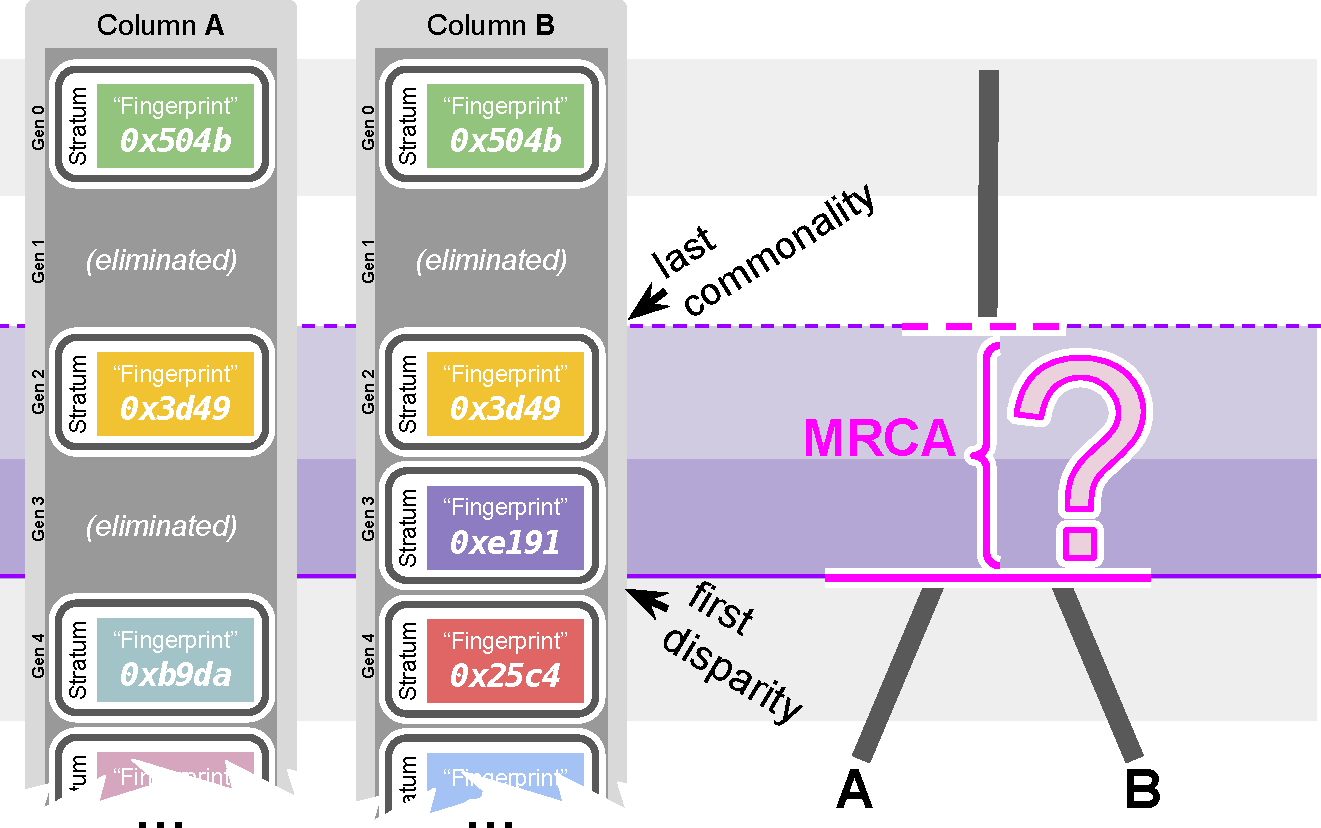
\includegraphics[width=\columnwidth]{img/column-comparison}
    \caption{
    Cartoon illustration of process to infer the generation of the most-recent common ancestor (MRCA) of two hereditary stratigraphic columns $A$ and $B$.
    Columns are aligned so that strata deposited at corresponding generations can be compared.
    Then, the first generation with disparate ``fingerprints'' is determined.
    (If a particular generation's strata have been eliminated from one or both columns or have not yet been deposited on one column, then no comparison is performed at that generation.)
    This provides a hard upper bound on the generation of the MRCA: these strata \textit{must} have been deposited along separate lines of descent.
    Then, searching backward for first commonality preceding that disparity provides a soft lower bound on the generation of the MRCA: these strata evidence common ancestry but \textit{might} collide by chance.
    (If a narrow ``fingerprint'' differentia like a single bit is used with plausible collision probability, a lower bound can be established by continuing to search backward until the probability of $k$ successive spurious collisions is sufficiently unlikely.)
    This process yields certainty about the phylogenetic relationship between $A$ and $B$ shown at right above (i.e., common) and below (i.e., diverged) the MRCA bounds.
    }
  \label{fig:column-comparison}
\end{figure}
